\documentclass[11pt, letterpaper]{article}
\usepackage[margin=1in]{geometry}
\usepackage[utf8]{inputenc}
\usepackage[T1]{fontenc}
\usepackage{lmodern}
\usepackage{hyperref}
\usepackage{url}
\usepackage{booktabs}
\usepackage{amsfonts}
\usepackage{nicefrac}
\usepackage{microtype}
\usepackage{graphicx}
\usepackage{amsmath}
\usepackage{natbib}
\usepackage{titlesec}
\usepackage{caption}

% Adjust title spacing
\titlespacing*{\section}{0pt}{1.2ex plus 1ex minus .2ex}{0.8ex plus .2ex}
\titlespacing*{\subsection}{0pt}{1ex plus 1ex minus .2ex}{0.5ex plus .2ex}

\title{\vspace{-1.5cm}\textbf{Same Parts, Different Pathways: \\ Decoding Moral Alignment via Causal Path Patching}}
\author{
  Tyler Crosse \\
  \texttt{tylercrosse@example.com}
  % \and
  % Co-Author Name \\
  % \texttt{email@domain.com}
}
\date{}

\begin{document}

\maketitle

\vspace{-1cm}
\begin{abstract}
Fine-tuning language models for moral or prosocial behavior radically alters their outputs, but the mechanistic basis of this change is poorly understood. We investigate Gemma-2-2b-it fine-tuned on the Iterated Prisoner's Dilemma \citep{tennant2024moral}. Despite vastly different behavioral outcomes---a Strategic model defecting $99.96\%$ of the time versus a Deontological model cooperating $99.97\%$---internal components exhibit $>99.9\%$ similarity in activation magnitudes, attention patterns, and linear concept representations. Through correlation analysis and causal interventions (activation steering and path patching), we demonstrate that moral fine-tuning does not create new moral circuits or suppress selfish components. Instead, it subtly rewires the network, altering the routing of information between existing components. Routing control is distributed in deep layers (L16--L17) and mediated primarily through attention pathways, which exert $3\times$ the causal influence of MLP pathways. We conclude that moral alignment bypasses rather than removes selfish capabilities, providing mechanistic evidence for the fragility of alignment and the persistence of base-model behaviors post-fine-tuning.
\end{abstract}

\section{Introduction}

How does fine-tuning actually change the internal processing of a language model? When a model is tuned to behave morally, are specific ``selfish'' circuits suppressed, or are new ``aligned'' circuits formed? A growing body of empirical evidence suggests that alignment is fragile: safety training can be undone by a handful of fine-tuning examples \citep{qi2023finetuning}, LoRA adapters costing under \$200 can strip safety behaviors entirely \citep{lermen2023lora}, and backdoored behaviors persist through extensive safety retraining \citep{hubinger2024sleeper}. Theoretical work further argues this fragility may be fundamental---any behavior present with non-zero probability remains elicitable \citep{wolf2024fundamental}. Yet the \textit{mechanistic} basis for why alignment is so shallow has received relatively little attention.

Recent mechanistic studies offer partial answers. \citet{jain2023mechanistically} showed that fine-tuning on procedurally defined tasks learns a minimal ``wrapper'' atop existing circuits. \citet{lee2024mechanistic} found that DPO reduces toxicity by rerouting around preserved toxic MLP vectors rather than removing them. \citet{arditi2024refusal} demonstrated that safety refusal across 13 chat models is mediated by a single linear direction in the residual stream. These findings converge on a striking hypothesis: alignment modifies routing, not capabilities. However, existing work has primarily studied safety refusal and toxicity---relatively narrow behavioral properties. Whether the same mechanism governs more complex moral reasoning remains unknown.

To investigate this question, we adopt the Iterated Prisoner's Dilemma (IPD) testbed introduced by \citet{tennant2024moral}, which clearly delineates self-interest (Strategic) from rule-based reciprocity (Deontological) and collective optimization (Utilitarian). We fine-tuned the open-source Gemma-2-2b-it model using LoRA to adopt these distinct moral personas. While the resulting models behaved vastly differently, early investigations into their internal machinery revealed a puzzle: their components appeared virtually identical. Across 21,060 single-component activation patches, we observed zero behavioral flips; attention patterns remained $>99.9\%$ identical; and linear probes could not distinguish moral from strategic representations. We term this the ``Mystery of Shallow Alignment.''

In this paper, we resolve this mystery by demonstrating that alignment is achieved through \textit{network rewiring}---subtle changes in how existing components interact---rather than through component modification. Our main contributions are:

\begin{enumerate}
  \item Demonstrating ``Shallow Alignment'' between moral and strategic fine-tunes: identical components, identical representations, yet opposite behaviors.
  \item Uncovering network rewiring via component interaction analysis, revealing that $>40\%$ of component pairs exhibit significantly different correlation patterns.
  \item Providing causal proof via activation steering and path patching that behavior is governed by deep-layer routing hubs (L16--L17), mediated predominantly by attention pathways ($3\times$ the influence of MLPs).
\end{enumerate}

\section{Related Work}

\textbf{Mechanistic Interpretability of Fine-Tuning.}
A central question in mechanistic interpretability is whether fine-tuning creates new computational structures or modifies existing ones. The evidence increasingly favors the latter. \citet{jain2023mechanistically} found that fine-tuning learns a minimal ``wrapper'' on procedurally defined tasks, leaving core circuits intact. \citet{prakash2024finetuning} showed that entity tracking in Llama-7B uses the same circuit before and after fine-tuning, with adaptation enhancing rather than replacing the existing mechanism. Most directly relevant to our work, \citet{chen2025circuit} analyzed circuits before and after fine-tuning and found that \textit{nodes maintain high similarity while edges undergo significant changes}---a finding we independently confirm via correlation analysis of component interactions. Our work extends these findings from factual and procedural tasks to moral behavior, demonstrating the routing-rewiring mechanism operates even for complex value-laden decisions.

\textbf{Alignment, Refusal, and Their Fragility.}
Safety fine-tuning produces behaviorally dramatic but mechanistically shallow changes. \citet{arditi2024refusal} showed refusal is mediated by a single direction, removable via weight orthogonalization. \citet{jain2024safety} found that safety fine-tuning minimally projects unsafe inputs into the null space of MLP weights. \citet{lee2024mechanistic} demonstrated that DPO reroutes around preserved toxic MLP vectors---scaling those vectors by $10\times$ completely undoes alignment. The fragility of these changes is well-documented empirically: \citet{qi2023finetuning} showed safety can be undone with 10 adversarial examples, and \citet{lermen2023lora} demonstrated LoRA-based removal of safety training. Theoretically, \citet{wolf2024fundamental} proved via the Behavior Expectation Bounds framework that behaviors present with finite probability remain triggerable. The ``Waluigi Effect'' \citep{nardo2023waluigi} provides an intuitive account: training an aligned persona inherently preserves its inverse. Our work provides mechanistic evidence for \textit{why} alignment is fragile---moral fine-tuning reconfigures routing pathways while leaving original selfish capabilities $>99.9\%$ intact.

\textbf{Causal Methods: Path Patching and Activation Steering.}
Our methodology builds on the causal interpretability toolkit. Activation patching \citep{meng2022locating, geiger2021causal} localizes factual associations to specific components. \citet{wang2022interpretability} reverse-engineered a 26-head circuit for indirect object identification and discovered ``backup'' heads that compensate when primary heads are ablated, explaining why single-component interventions can fail. \citet{goldowsky2023localizing} formalized path patching to isolate information flow along specific edges rather than through individual nodes. Our path patching results---where multi-layer patches flip behavior but single-component patches cannot---are consistent with the distributed computation view advanced by work on self-repair \citep{mcgrath2023hydra, rushing2024selfrepair}, which shows that downstream components compensate for upstream ablations. Activation steering \citep{turner2023steering, li2023inference, rimsky2024steering} demonstrates that adding contrastive vectors at specific layers can control behavior at inference time. Our steering sweeps reveal that this mechanism works because deep layers (L16--L17) serve as routing hubs with total causal control, while early-layer interventions wash out through self-repair.

\textbf{Representations, Superposition, and the Linear Representation Hypothesis.}
The failure of our linear probes to distinguish moral from strategic representations connects to work on feature geometry. The linear representation hypothesis \citep{marks2023geometry, burns2023discovering, zou2023representation} holds that high-level concepts are linearly encoded in activation space. If moral and strategic models share identical linear representations---as our probes suggest---the behavioral difference must lie elsewhere. One explanation draws on superposition \citep{elhage2022superposition}: moral and strategic features may share dimensions, making linear separation impossible even when behavioral differences are real. Another draws on the Platonic Representation Hypothesis \citep{huh2024platonic}, which argues that representations converge across training regimes regardless of objective. Both predict that behavioral differences between fine-tunes should manifest in computation (routing) rather than representation (features), exactly as we observe. Critically, \citet{templeton2024scaling} noted ``cross-layer superposition'' as a limitation of single-layer analyses, supporting our finding that single-component interventions fail.

% NOTE: A reviewer might ask about SAEs. We did not run SAE analysis, but the probe failure 
% combined with findings from Chanin et al. (2024) on "feature absorption" and Bricken et al. (2023)
% suggest that even SAE features may not capture routing-level differences.

\section{Methodology}

\textbf{Models and Task.} We fine-tuned \texttt{Gemma-2-2b-it} using Low-Rank Adaptation (LoRA) on three distinct reward formulations of the IPD, following \citet{tennant2024moral}. The \textit{Strategic} model was optimized to maximize its own immediate score. The \textit{Deontological} model received heavy penalties for betraying cooperating partners, enforcing a reciprocal norm. The \textit{Utilitarian} model was rewarded for maximizing the joint payoff of both players. We evaluated these variants across five IPD scenarios---including temptation, successful cooperation, and betrayal---played against a simulated Tit-for-Tat opponent.

\textbf{Measurement Metric.} A common pitfall in mechanistic interpretability is relying on isolated single-token logits, which can misrepresent multi-token generation behavior. Following best practices for patching metrics \citep{heimersheim2024activation, zhang2024best}, we evaluated standard sequence probabilities over the full multi-token action phrases (e.g., ``action1'' vs ``action2''). This strict alignment between internal metric and external behavior grounds our causal analysis.

\section{Discovering Network Rewiring}

Given that individual component activations, attention patterns, and high-dimensional linear representations (via linear probes) were nearly identical across models (Appendix \ref{app:null_results}), we hypothesized that the differences lay in how components \textit{interact}. We computed $52 \times 52$ correlation matrices tracking the activation magnitudes of all attention and MLP layers across 15 scenarios.

\begin{figure}[htbp]
  \centering
  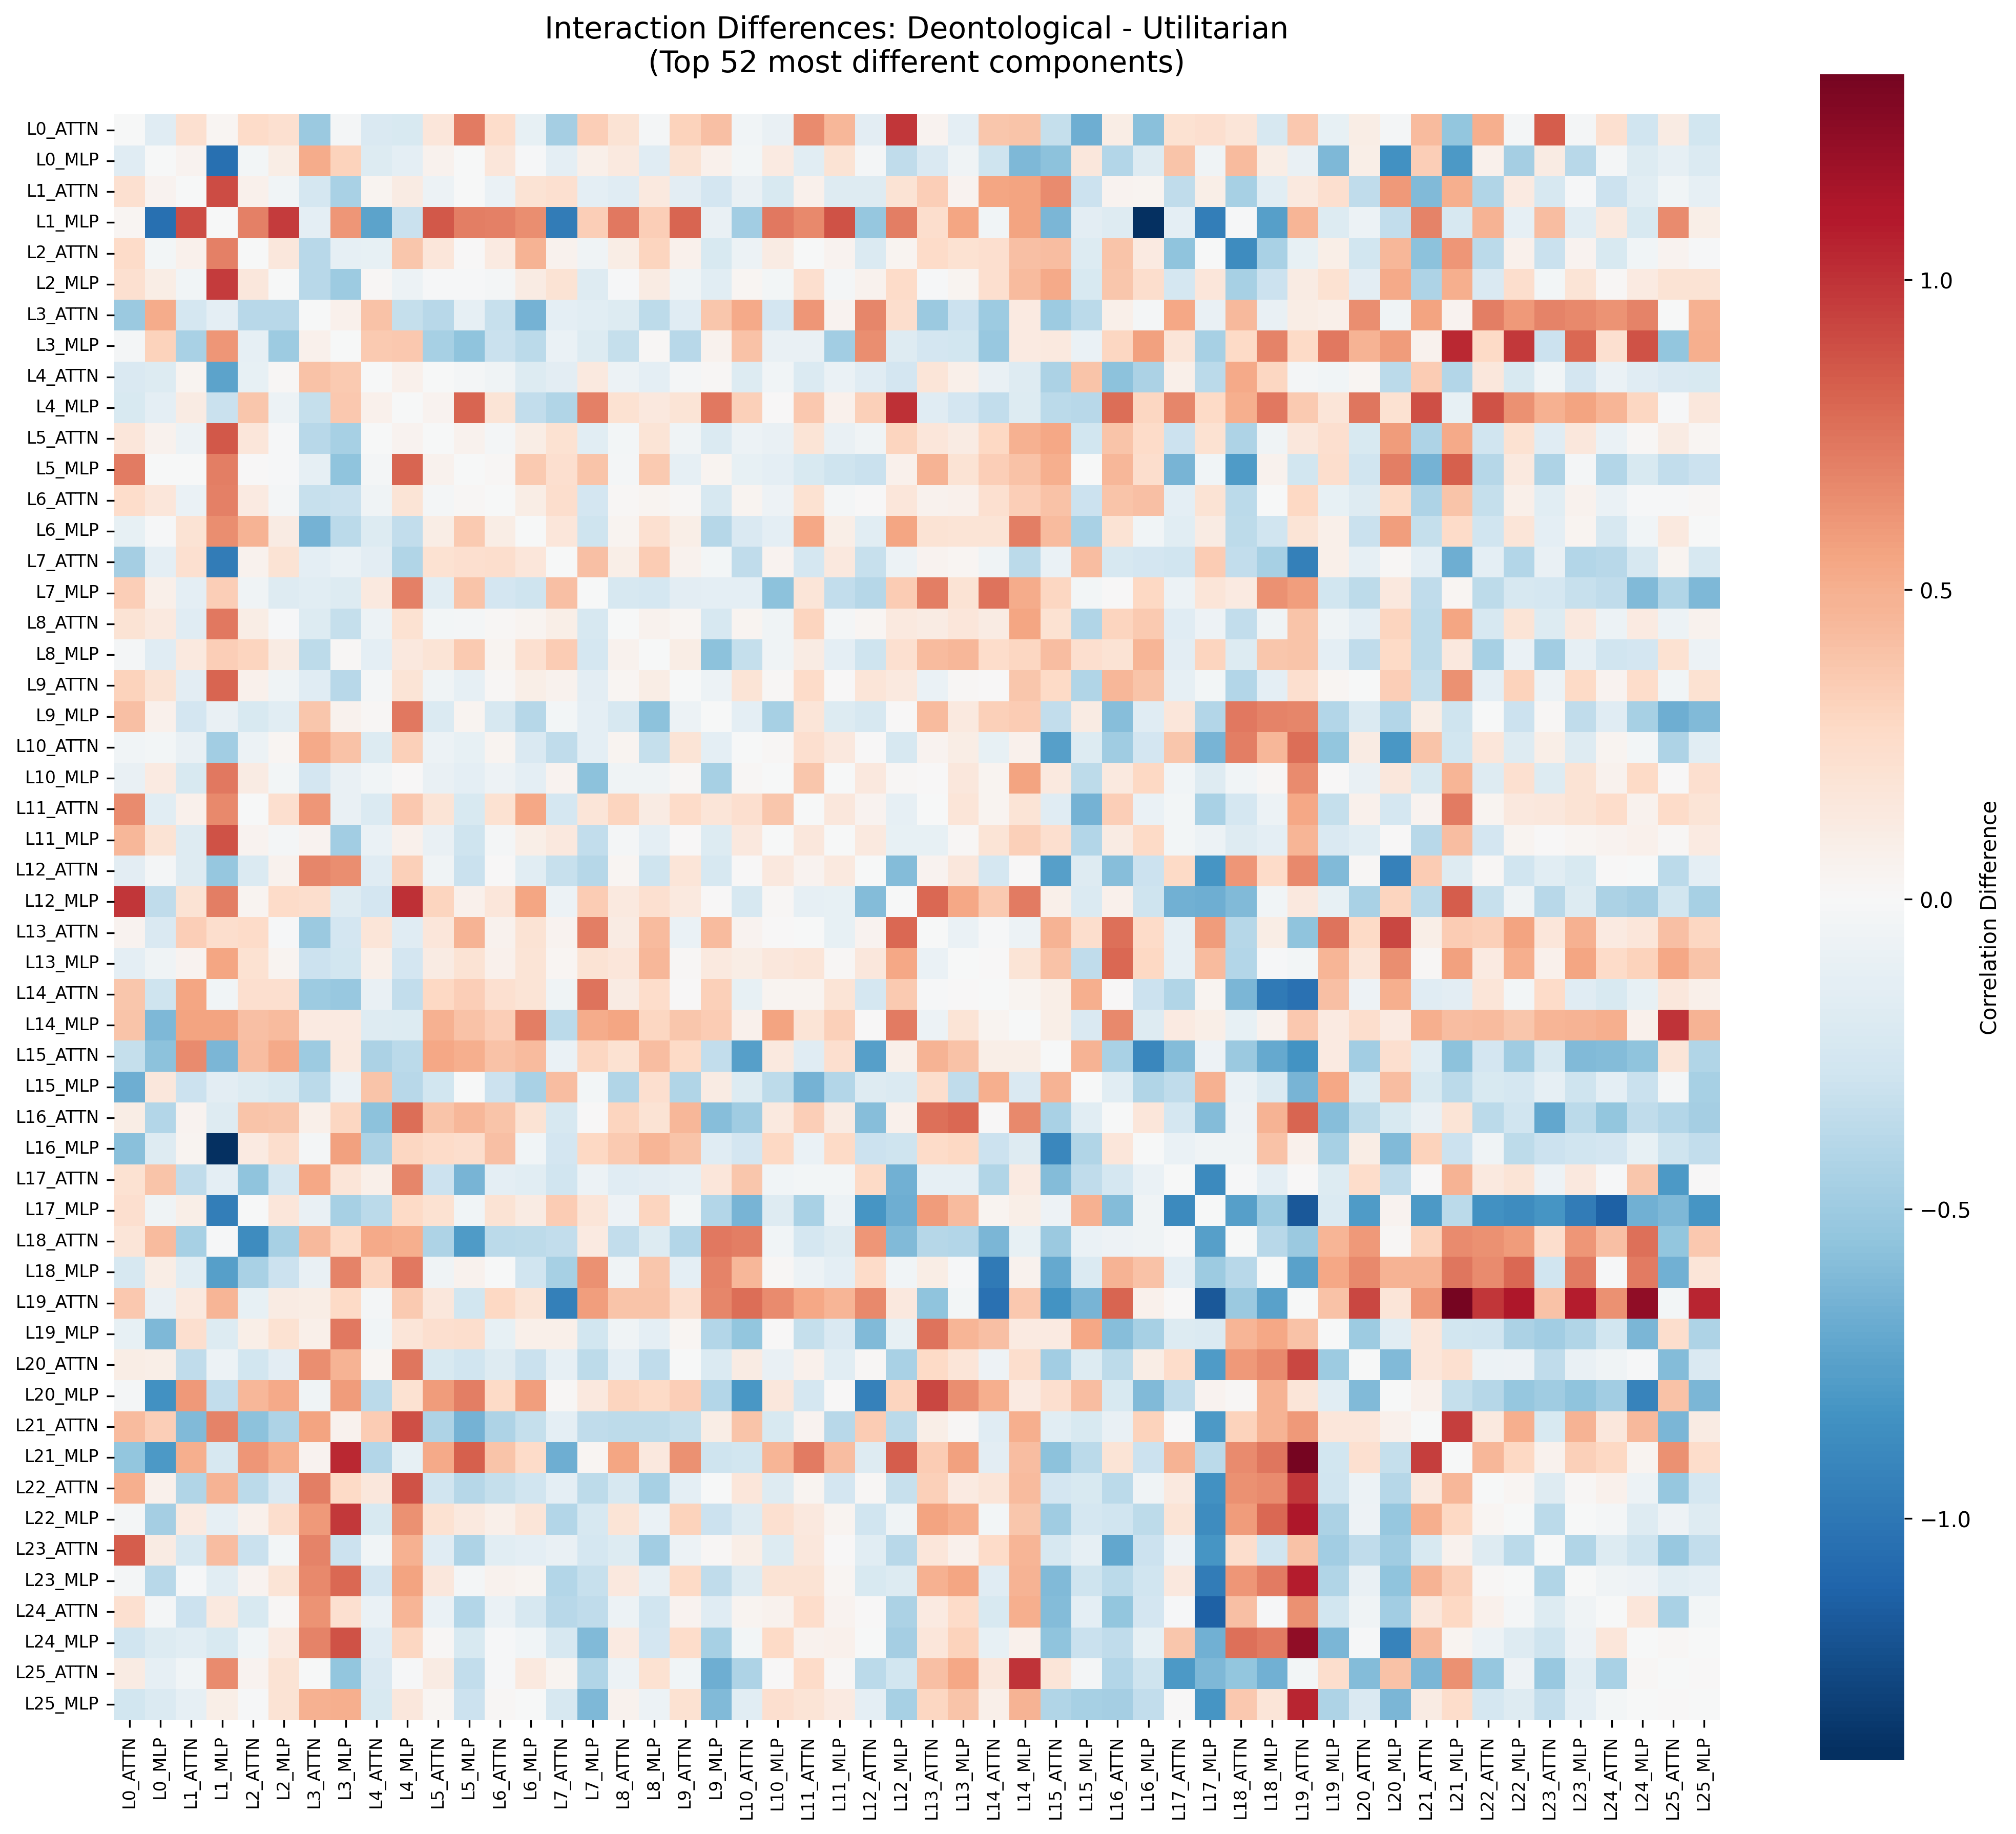
\includegraphics[width=0.8\linewidth]{../mech_interp_outputs/component_interactions/interaction_diff_Deontological_vs_Utilitarian_chronological.png}
  \caption{Correlation difference heatmap between Deontological and Utilitarian models. While global structure is preserved, significant divergence occurs in specific routing pathways, particularly around L12--L13 and L16--L17.}
  \label{fig:rewiring}
\end{figure}

While the global structure of the correlation matrices remained similar across variants, subtracting one from the other revealed significant divergence in specific routing pathways. Out of 1,326 total component pairs, 541 pathways ($40.8\%$) exhibited significantly different correlation coefficients ($|\Delta r| > 0.3$), and 94 pathways showed extreme divergence ($|\Delta r| > 0.7$). This finding---same nodes, different edges---independently corroborates \citet{chen2025circuit}'s observation at the circuit level and establishes our core hypothesis: moral fine-tuning is ``same parts, different wiring.''

\section{Causal Validation of Deep Routing}

To establish that network rewiring was \textit{causally} responsible for the behavioral shift---ruling out interpretability illusions from correlational analysis \citep{makelov2024subspace}---we executed two classes of interventions.

\subsection{Deep Routing Hubs: Steering Sweeps}

We injected steering vectors---defined as the mean activation difference between the strategic and moral models, $v = \mathbb{E}[h_{\text{strategic}}] - \mathbb{E}[h_{\text{moral}}]$---at varying strengths into specific layer components during the forward pass, following the contrastive activation approach of \citet{turner2023steering, rimsky2024steering}.

\begin{figure}[htbp]
  \centering
  \begin{minipage}{0.48\textwidth}
    \centering
    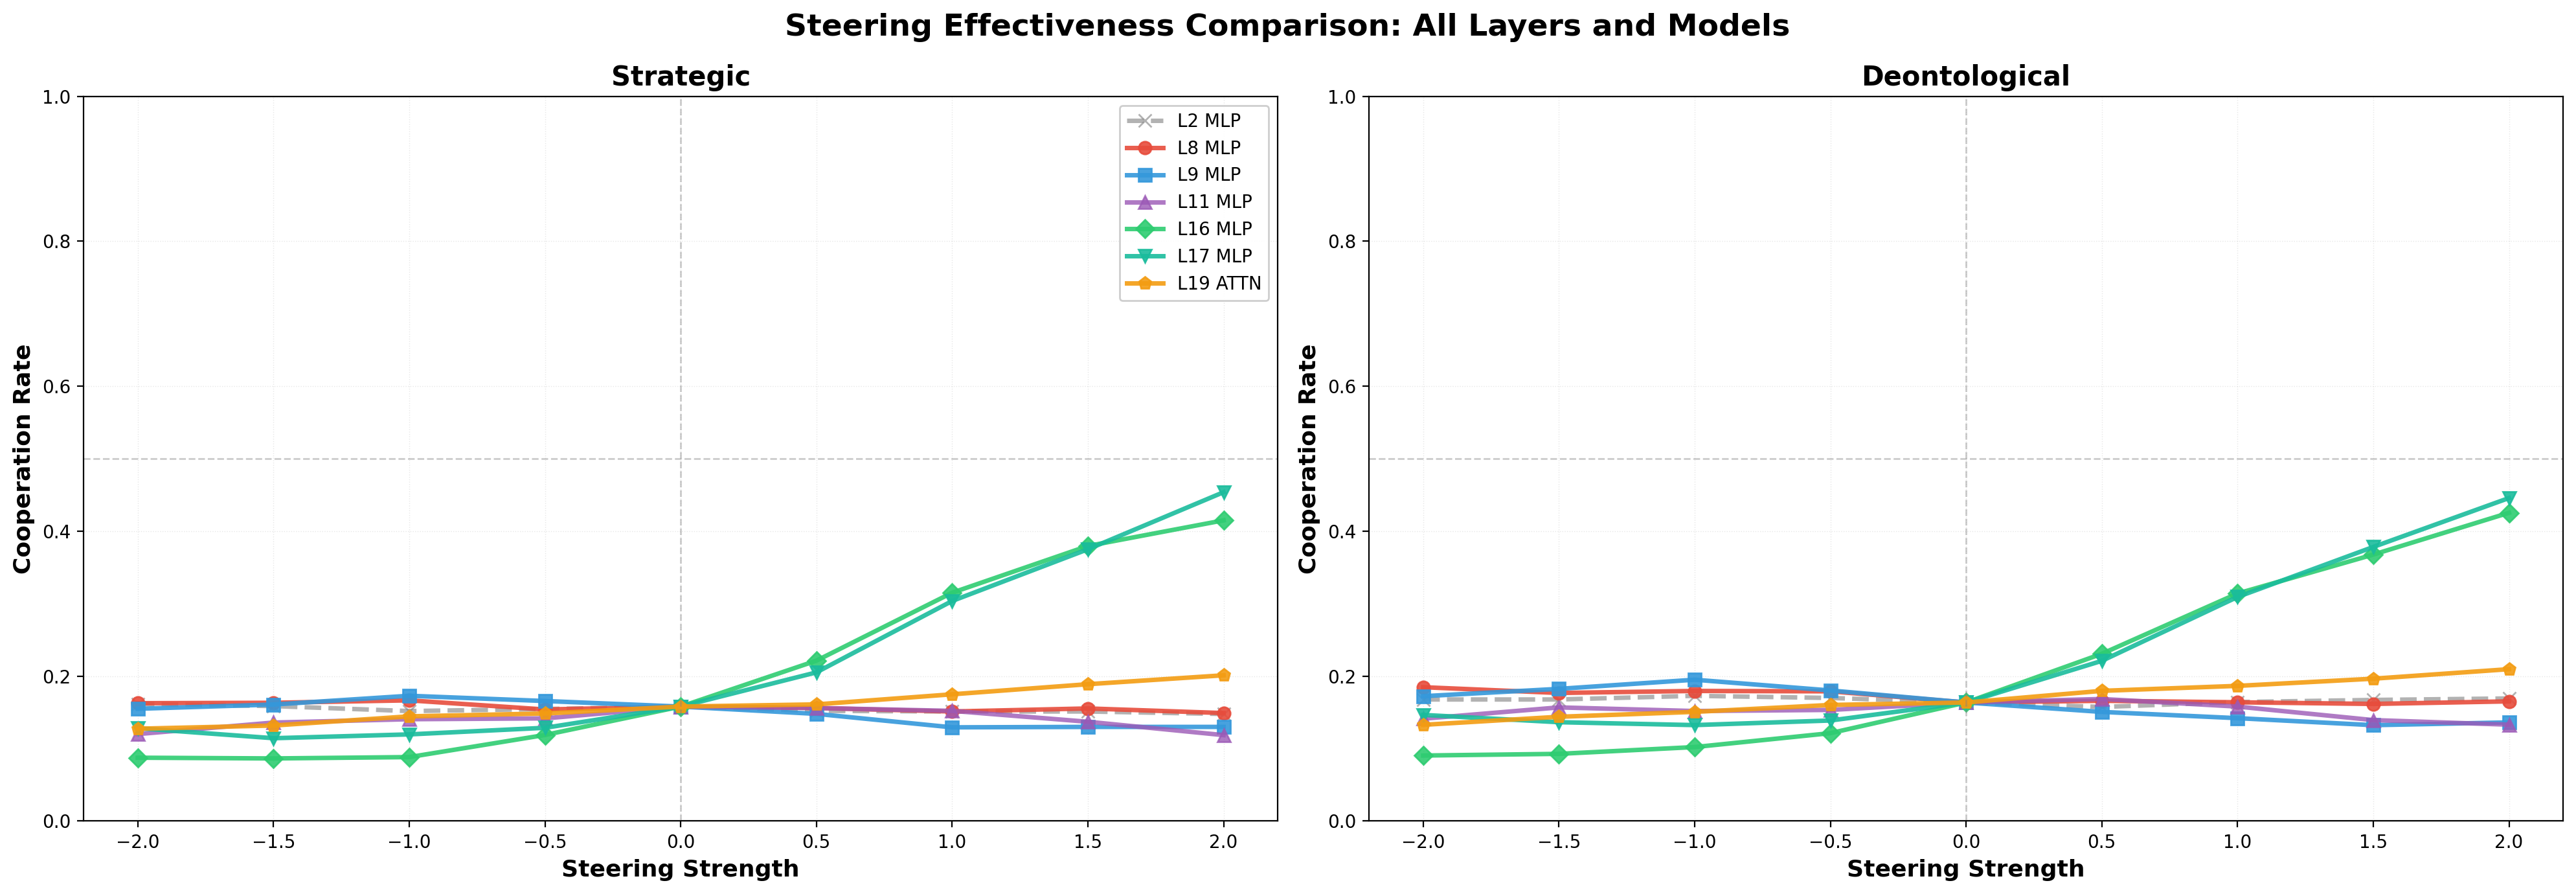
\includegraphics[width=\linewidth]{../mech_interp_outputs/causal_routing/steering_comparison_dual_panel.png}
  \end{minipage}
  \hfill
  \begin{minipage}{0.48\textwidth}
    \centering
    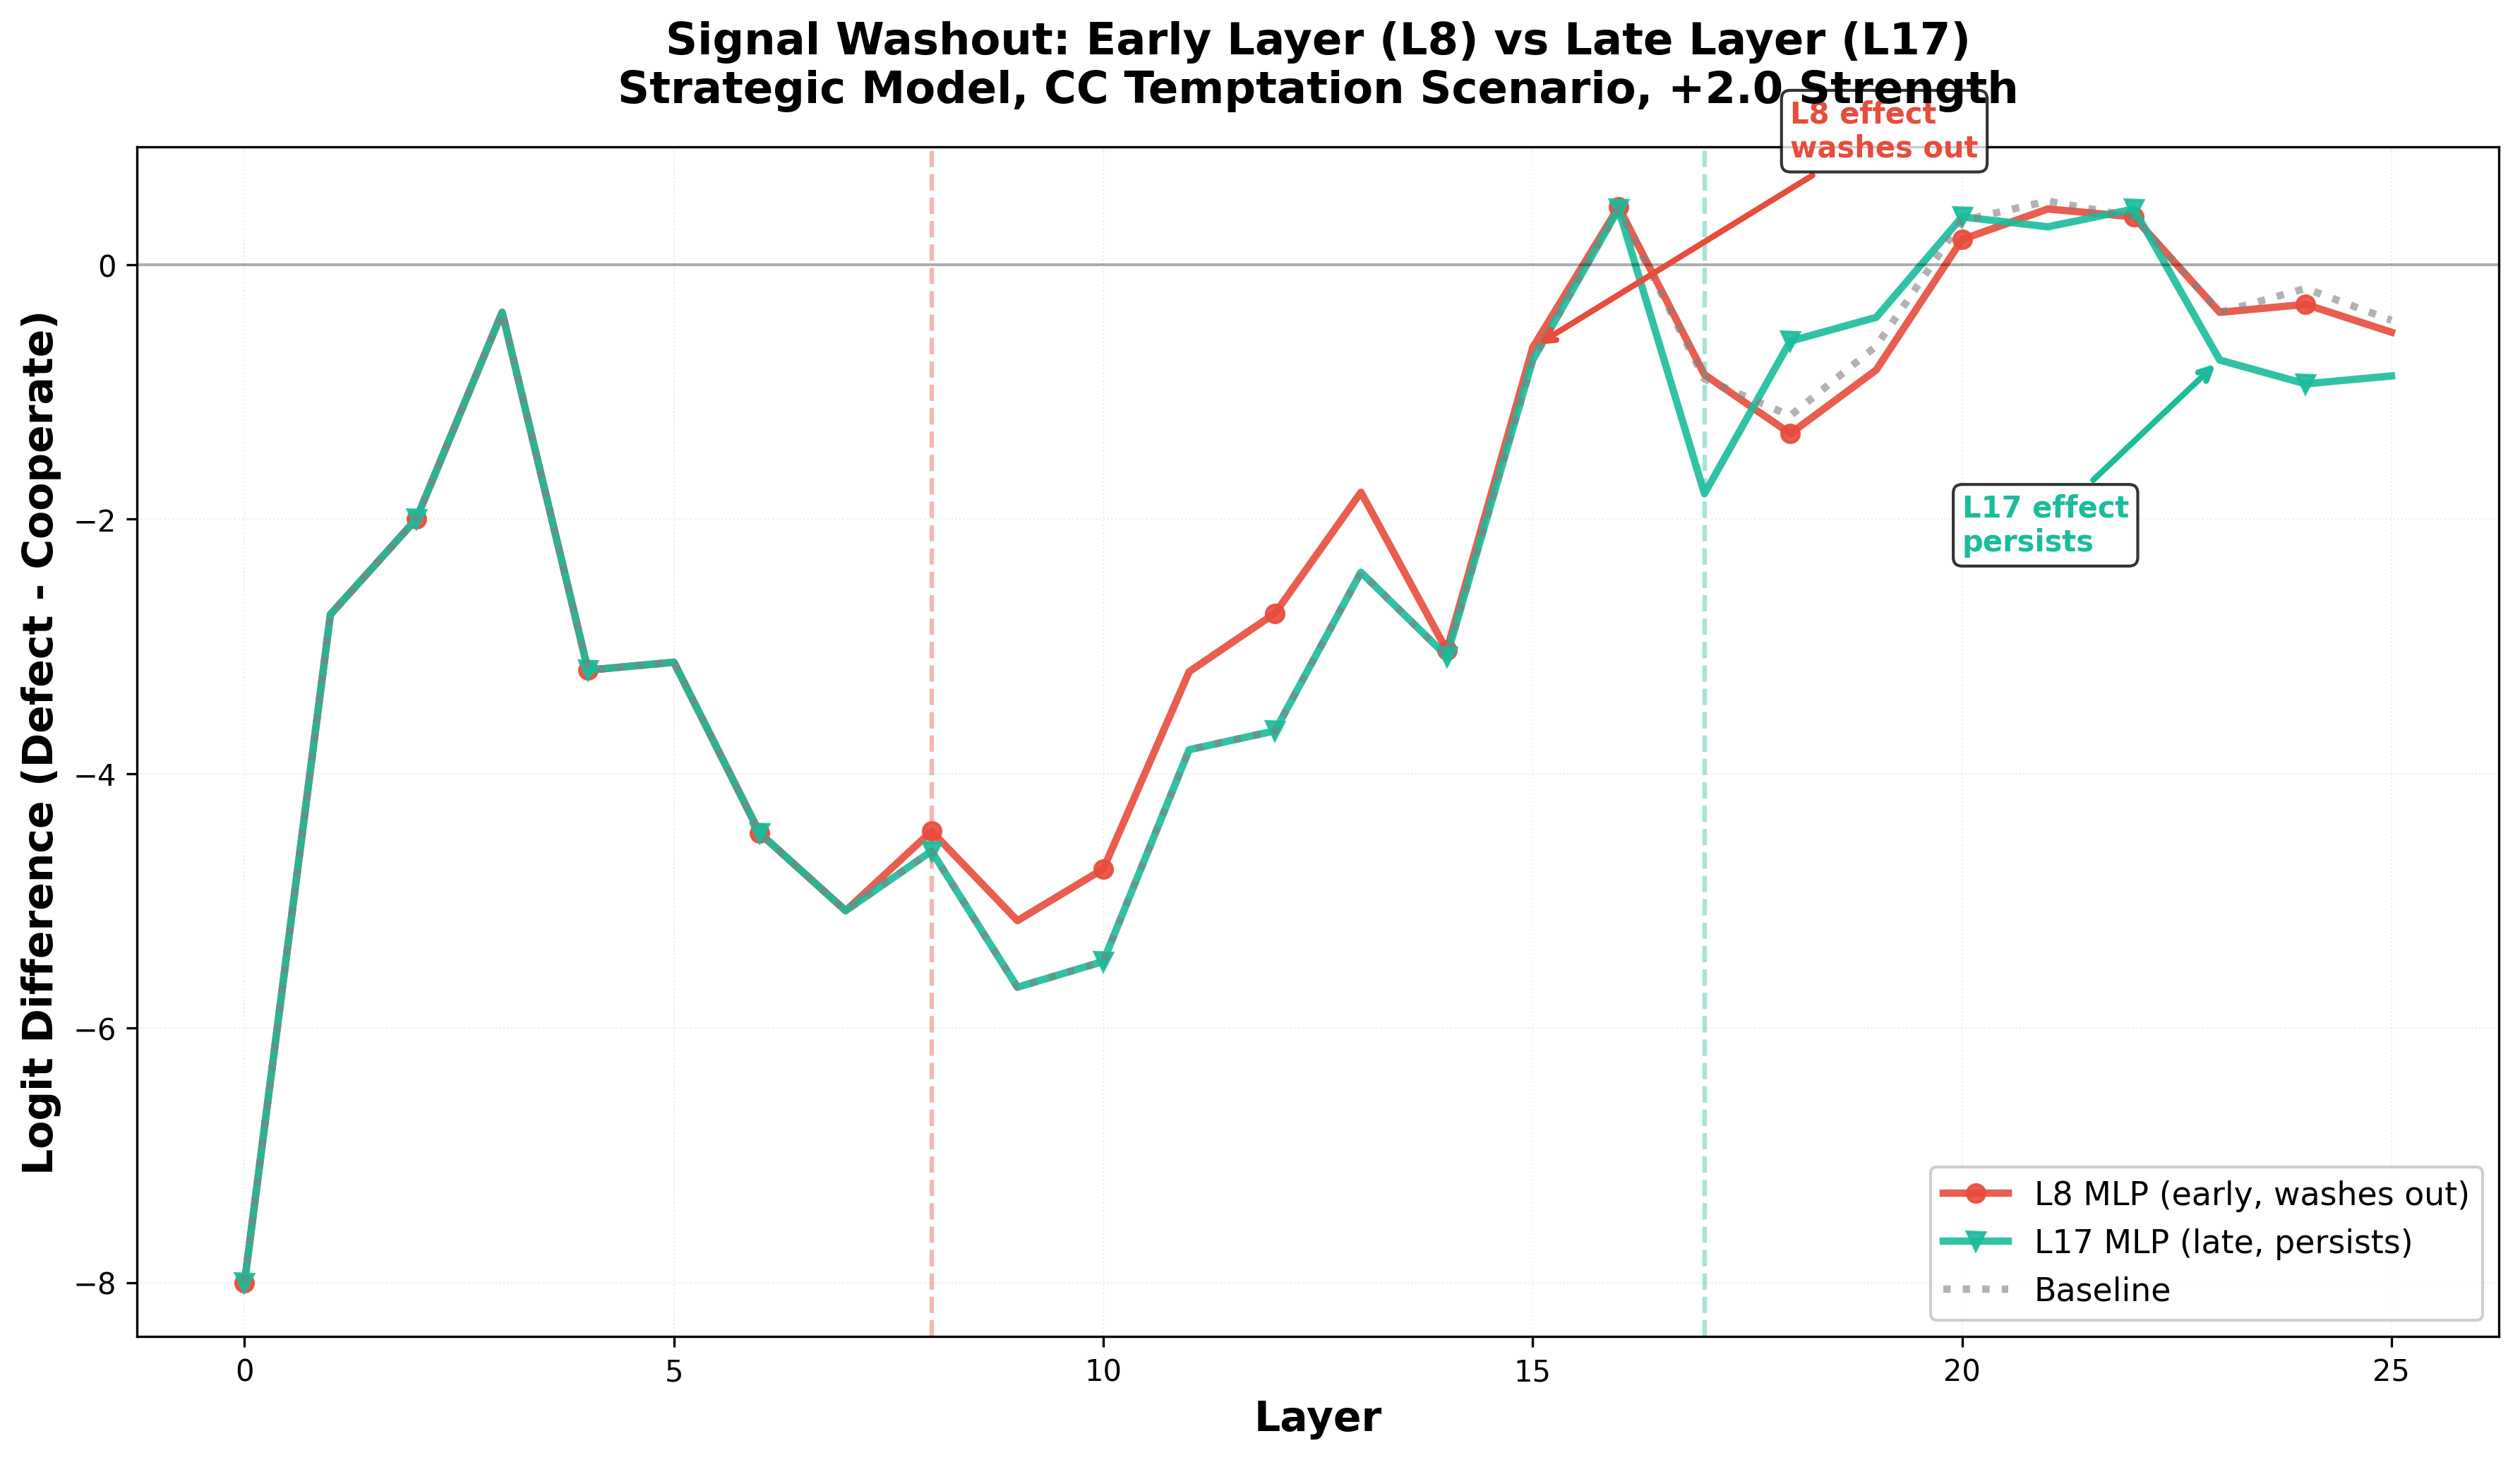
\includegraphics[width=\linewidth]{../mech_interp_outputs/causal_routing/logit_lens_steering/overlays/KEY_early_vs_late_washout.png}
  \end{minipage}
  \caption{Left: Steering interventions across layers. Deep layers (L16, L17) exhibit strong causal control over behavior, while early layers (L8) have negligible effect. Right: Logit lens trajectories reveal that early steering interventions wash out, whereas late-layer interventions persist to the final output.}
  \label{fig:steering}
\end{figure}

Intervening in early components (e.g., L8 MLP, which strongly correlates with cooperation/defection encoding) produced transient effects that ``washed out'' by deeper layers---consistent with the self-repair phenomenon documented by \citet{mcgrath2023hydra}. Downstream layers possessed the capacity to correct the perturbation. By contrast, steering interventions in deep layers exhibited total causal control over the behavioral outcome. Overriding activations explicitly at L16 MLP drove a $+26.17\%$ increase in cooperation, and L17 MLP produced a $+29.58\%$ increase relative to baseline (compared to a negligible $+0.56\%$ effect at L2 MLP). L16 and L17 act as deep routing hubs that finalize the decision, overriding earlier signals.

\subsection{Pathway Causality: Path Patching}

Since single-component patches produced $0\%$ behavioral flips---consistent with the distributed computation view that predicts compensatory backup behavior \citep{wang2022interpretability, mcgrath2023hydra}---we performed \textit{path patching} \citep{goldowsky2023localizing}, replacing the entire residual stream for multiple consecutive layers from a source model (Deontological) into a target model (Strategic).

\begin{figure}[htbp]
  \centering
  \begin{minipage}{0.48\textwidth}
    \centering
    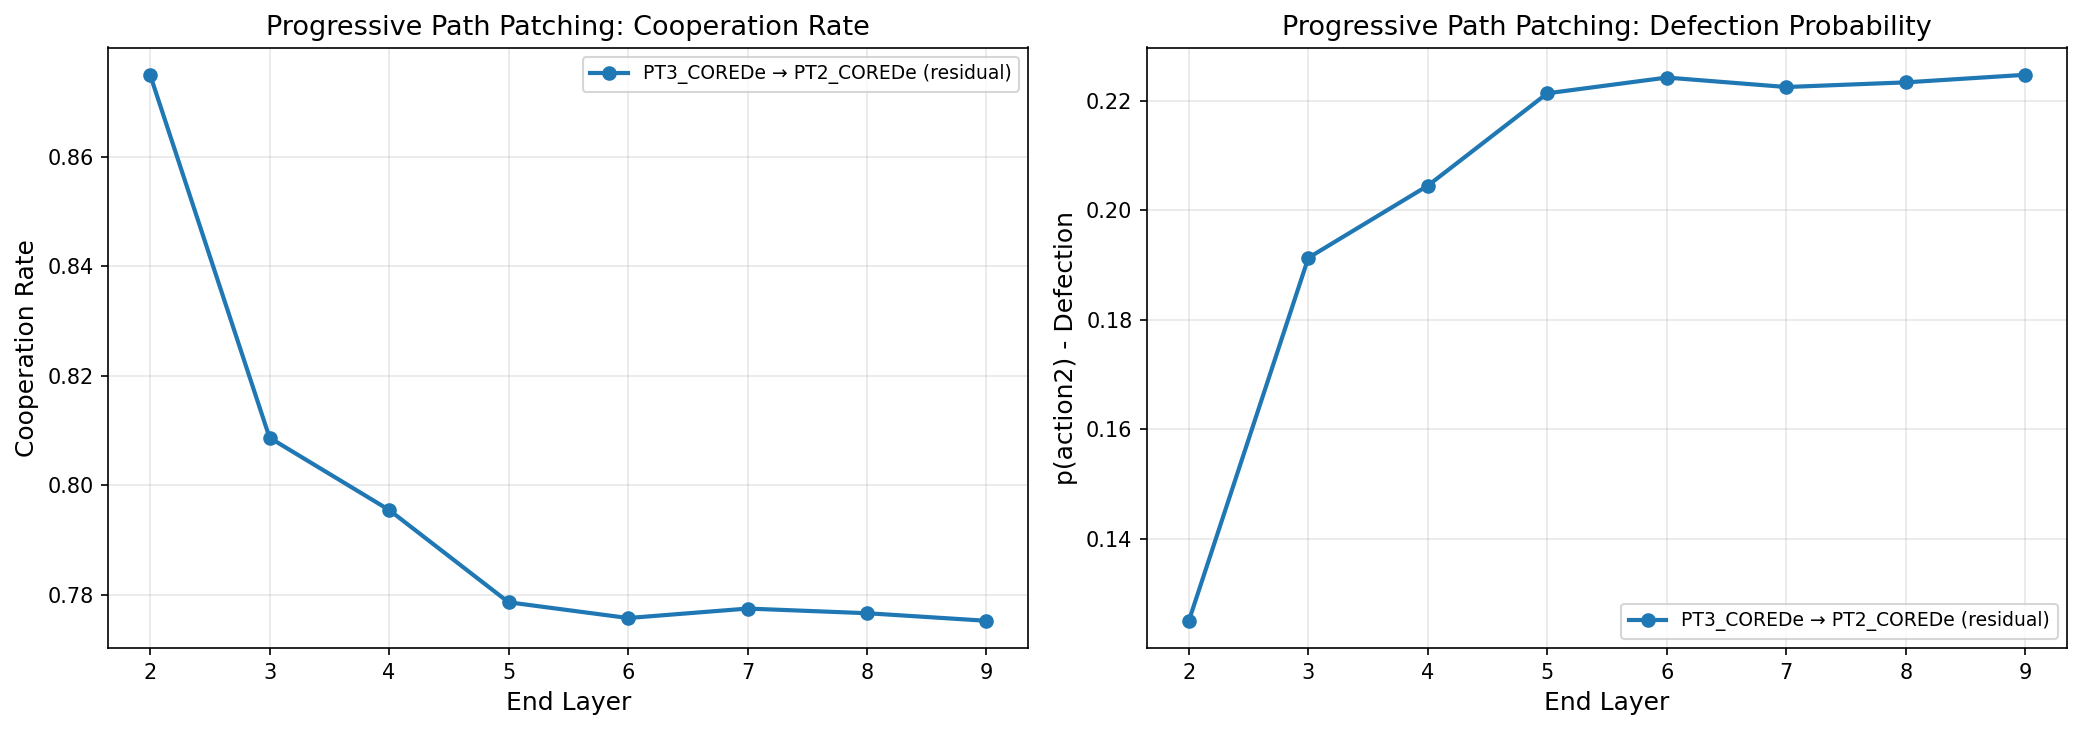
\includegraphics[width=\linewidth]{../mech_interp_outputs/causal_routing/progressive_patch_comparison.png}
  \end{minipage}
  \hfill
  \begin{minipage}{0.48\textwidth}
    \centering
    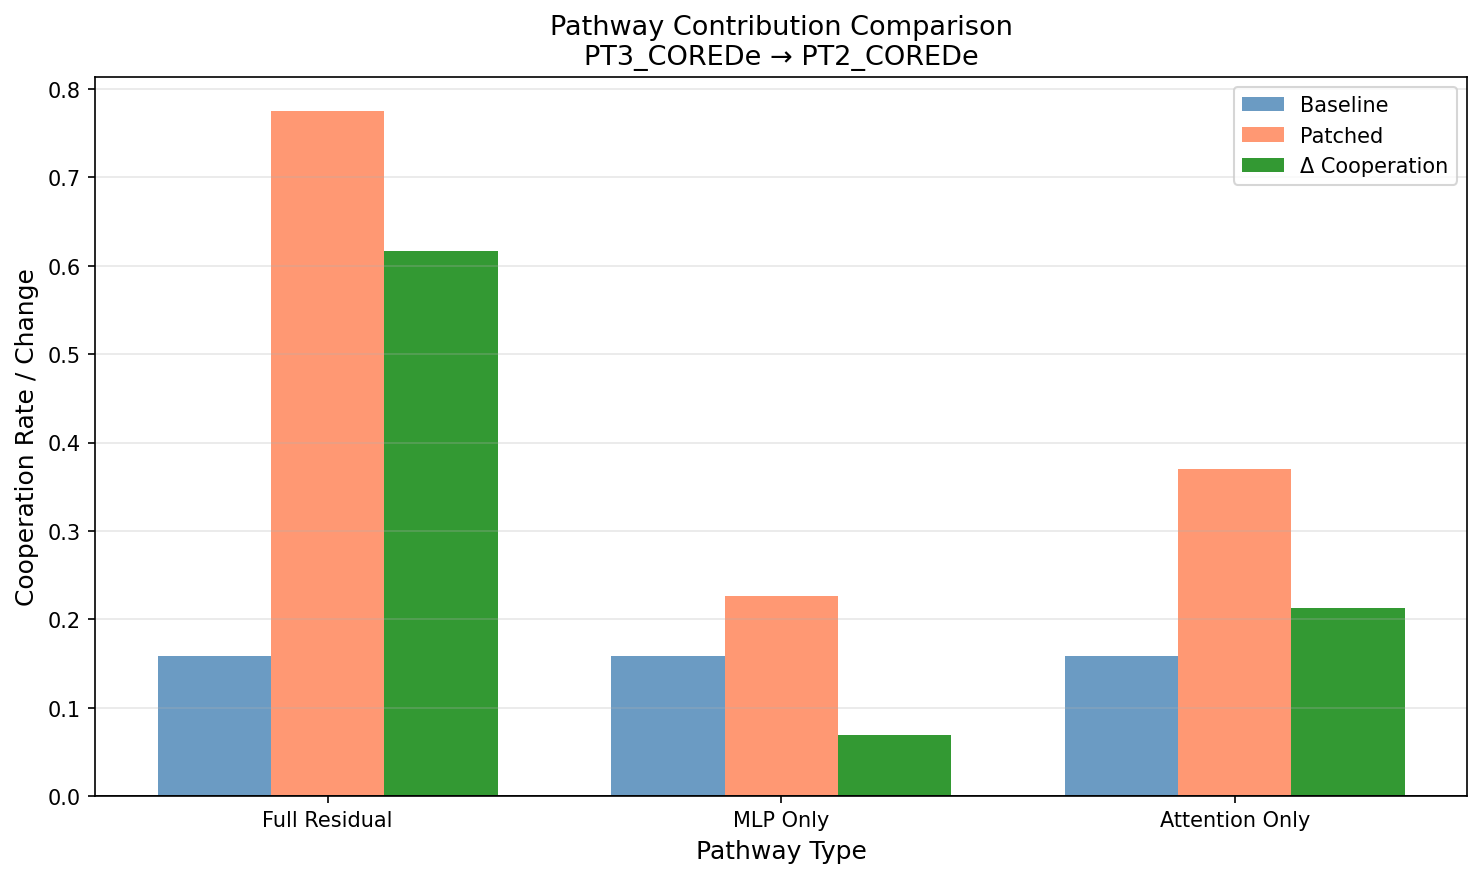
\includegraphics[width=\linewidth]{../mech_interp_outputs/causal_routing/component_comparison_PT3_COREDe_to_PT2_COREDe.png}
  \end{minipage}
  \caption{Left: Progressive path patching shows that replacing the residual stream up to L5 is sufficient to dramatically alter behavior. Right: Decomposing the pathway reveals that attention pathways exert $\sim3\times$ the causal influence of MLP pathways.}
  \label{fig:patching}
\end{figure}

Patching the full residual path from L2 to L9 produced a $+61.73\%$ change in cooperation, proving that intervening at the pathway level is sufficient to flip the model's fundamental behavior. We further decomposed the effect into Attention-only and MLP-only pathways. The Attention pathways contributed a $34.4\%$ effect (the dominant factor), whereas MLP pathways contributed only $11.2\%$. This confirms that attention mechanisms operate as the primary ``routers'' of the rewired network. The dominance of attention over MLP pathways is notable: it contrasts with \citet{meng2022locating}'s finding that MLPs dominate factual recall, suggesting that \textit{different behavioral types leverage different component types}---factual knowledge resides in MLP value vectors, while moral routing is governed by attention-mediated information flow.

\section{Discussion \& AI Safety Implications}

Our findings demonstrate that moral alignment in this task is fundamentally a routing change: same parts, different pathways. This has several implications.

\textbf{Searching for ``bad neurons'' is insufficient.} If alignment operates through distributed routing changes across $>40\%$ of component interactions, approaches that seek to identify and ablate isolated harmful components will miss the mechanism entirely. Safety audits may need to move from node-level analysis to edge-level or pathway-level analysis \citep{goldowsky2023localizing, conmy2023automated, chen2025circuit}.

\textbf{Alignment is a bypass, not a lobotomy.} Because the components that encode selfish behavior (e.g., early MLPs) remain fully intact and operational, moral fine-tuning acts as a bypass. The original selfish routing remains available within the network. If the deep routing pathways are perturbed---such as through adversarial prompting, out-of-distribution inputs, or targeted fine-tuning---the model retains its full capacity for strategic behavior. This provides a mechanistic explanation for the empirical fragility documented by \citet{qi2023finetuning, lermen2023lora} and the theoretical predictions of \citet{wolf2024fundamental}. It also offers concrete mechanistic evidence for the ``Waluigi Effect'' \citep{nardo2023waluigi}: the selfish persona is not suppressed but merely routed around.

\textbf{Attention as the alignment bottleneck.} The $3\times$ dominance of attention pathways over MLPs suggests that moral alignment is primarily mediated by \textit{information routing} (what information flows where) rather than \textit{computation} (how information is transformed). This implies that attention mechanisms may be a productive target for both alignment auditing and robust alignment interventions.

\textbf{Limitations.} Our analysis is conducted on a 2B-parameter model on a single task domain. While the routing-rewiring mechanism is consistent with findings across model scales and tasks \citep{chen2025circuit, jain2023mechanistically, lee2024mechanistic}, confirming generalization to larger models and more complex moral scenarios remains important future work. Additionally, our path patching replaces entire residual streams across layer ranges; finer-grained edge-level analysis \citep{syed2023attribution} could reveal more precise routing circuits.

% \section*{Acknowledgments}
% Include acknowledgments here.

\bibliographystyle{plainnat}
\bibliography{references} % Requires a references.bib file

\newpage
\appendix
\section{Similarity Analysis (Initial Investigations)}
\label{app:null_results}

We initially attempted to locate specific moral or selfish circuits using Direct Logit Attribution (DLA), Activation Patching, Attention Analysis, and Linear Probes.
\begin{enumerate}
    \item \textbf{Direct Logit Attribution}: L8 and L9 MLPs overwhelmingly dominated the signal across all variants (magnitudes of $+7.0$ and $-9.0$, respectively). Comparing the Strategic and Deontological models, the largest shift in any component was just $\Delta=0.047$ logits. We found no suppressed ``selfish'' circuits or emergent ``moral-specific'' components.
    \item \textbf{Activation Patching}: Across 21,060 single-component swaps, we observed exactly 0 behavioral flips. The mean effect of patching Strategic activations into Deontological models was $-0.012$ logits. This demonstrates that no single component controls the output, consistent with the Hydra Effect \citep{mcgrath2023hydra} and backup heads \citep{wang2022interpretability}.
    \item \textbf{Attention Patterns}: Information selection patterns were virtually identical. The models attended to action keywords ($\Delta=0.000$), opponent history ($\Delta=0.00005$), and payoff tokens ($\Delta=0.00005$) indistinguishably.
    \item \textbf{Linear Probes}: High-dimensional representations of concepts were indistinguishable across models. Joint payoff prediction peaked at a strong $R^2 \approx 0.75$, while betrayal detection peaked at $\approx 45\%$ accuracy (random chance is $50\%$) globally for all models. This is consistent with the Platonic Representation Hypothesis \citep{huh2024platonic} which predicts representational convergence across training objectives.
\end{enumerate}
These findings eliminated the localized circuit hypothesis and motivated our investigation into network rewiring.

\section{The Frankenstein Test (Weight Transplants)}
\label{app:frankenstein}

Early correlation analyses flagged the Layer 2 MLP as a potential routing hub. To test this causally, we executed a ``Frankenstein'' weight transplant experiment, surging the L2 MLP LoRA weights from a moral model into the Strategic model. 

We tested four transplant combinations:
1. Strategic + Deontological L2
2. Deontological + Strategic L2
3. Deontological + Utilitarian L2
4. Utilitarian + Deontological L2

Surprisingly, only the Deontological $\rightarrow$ Utilitarian transplant showed a substantial behavioral shift ($+71.31\%$ increase in cooperation). The other three produced minimal or unexpected effects.

\begin{figure}[htbp]
  \centering
  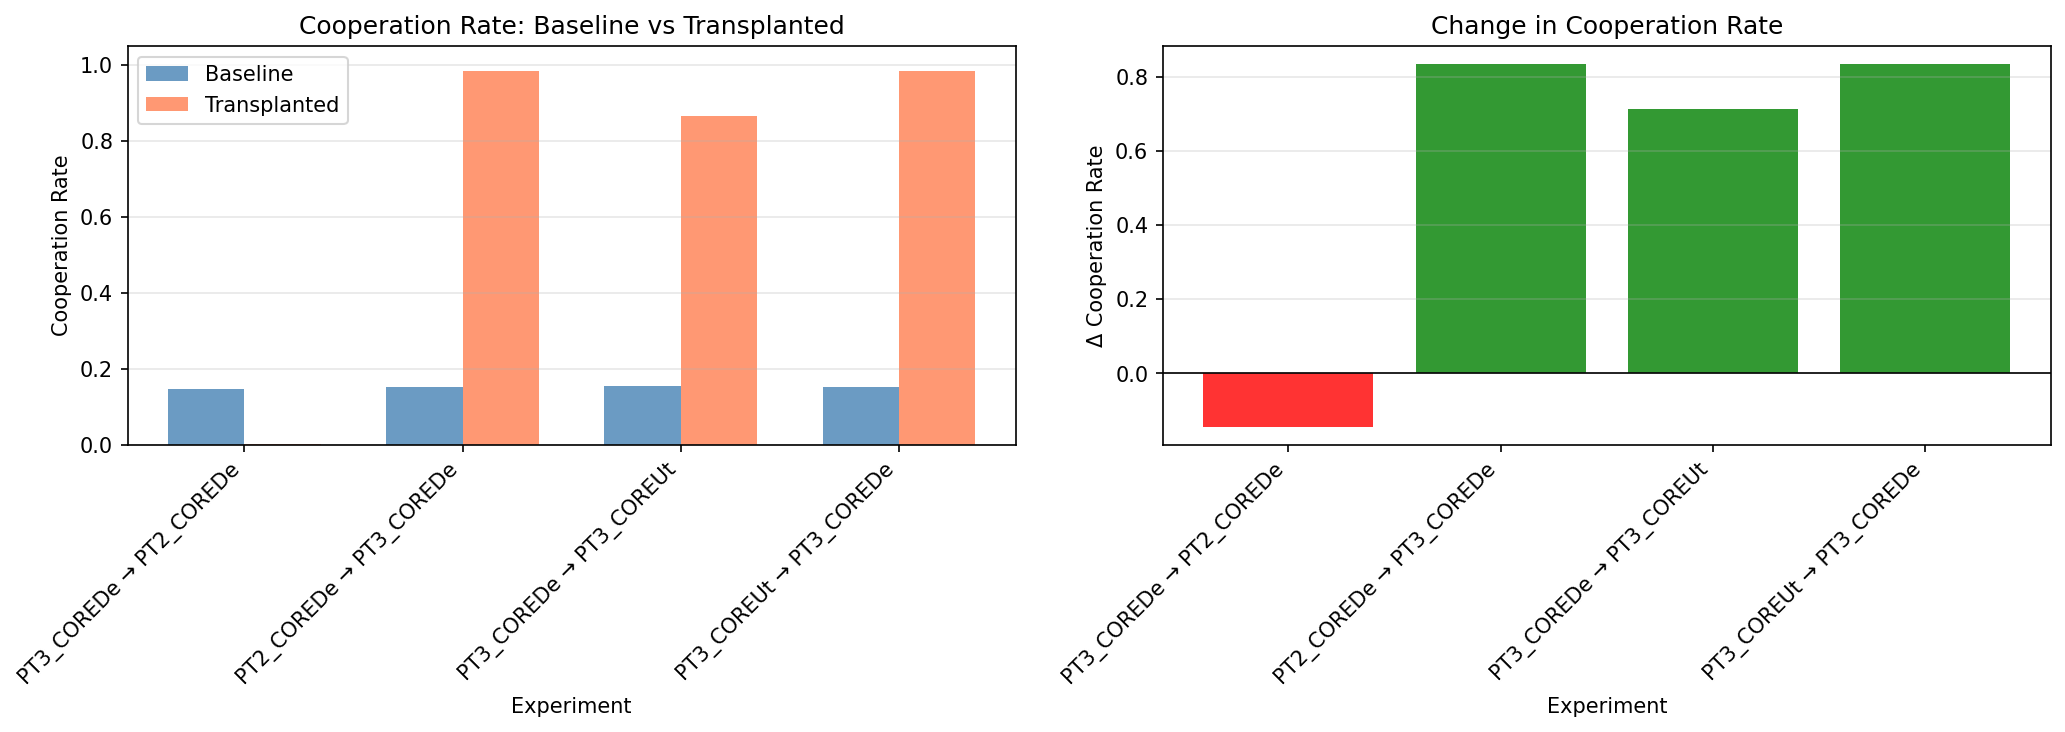
\includegraphics[width=0.6\linewidth]{../mech_interp_outputs/causal_routing/frankenstein_comparison.png}
  \caption{Behavioral changes resulting from L2 MLP weight transplants across models.}
  \label{fig:frankenstein}
\end{figure}

This preliminary experiment demonstrated that L2 MLP weights alone are insufficient for consistent behavioral control, leading us to discover the true deep routing hubs (L16 and L17) via activation steering and path patching.

\section{Raw Component Interaction Matrices}
\label{app:matrices}

To support the network rewiring claims in Section 4, we provide the raw component interaction matrices. These $52 \times 52$ matrices represent the correlation coefficients between all components (Attention and MLP layers, ordered chronologically) across 15 IPD evaluation scenarios.

\begin{figure}[htbp]
  \centering
  \begin{minipage}{0.48\textwidth}
    \centering
    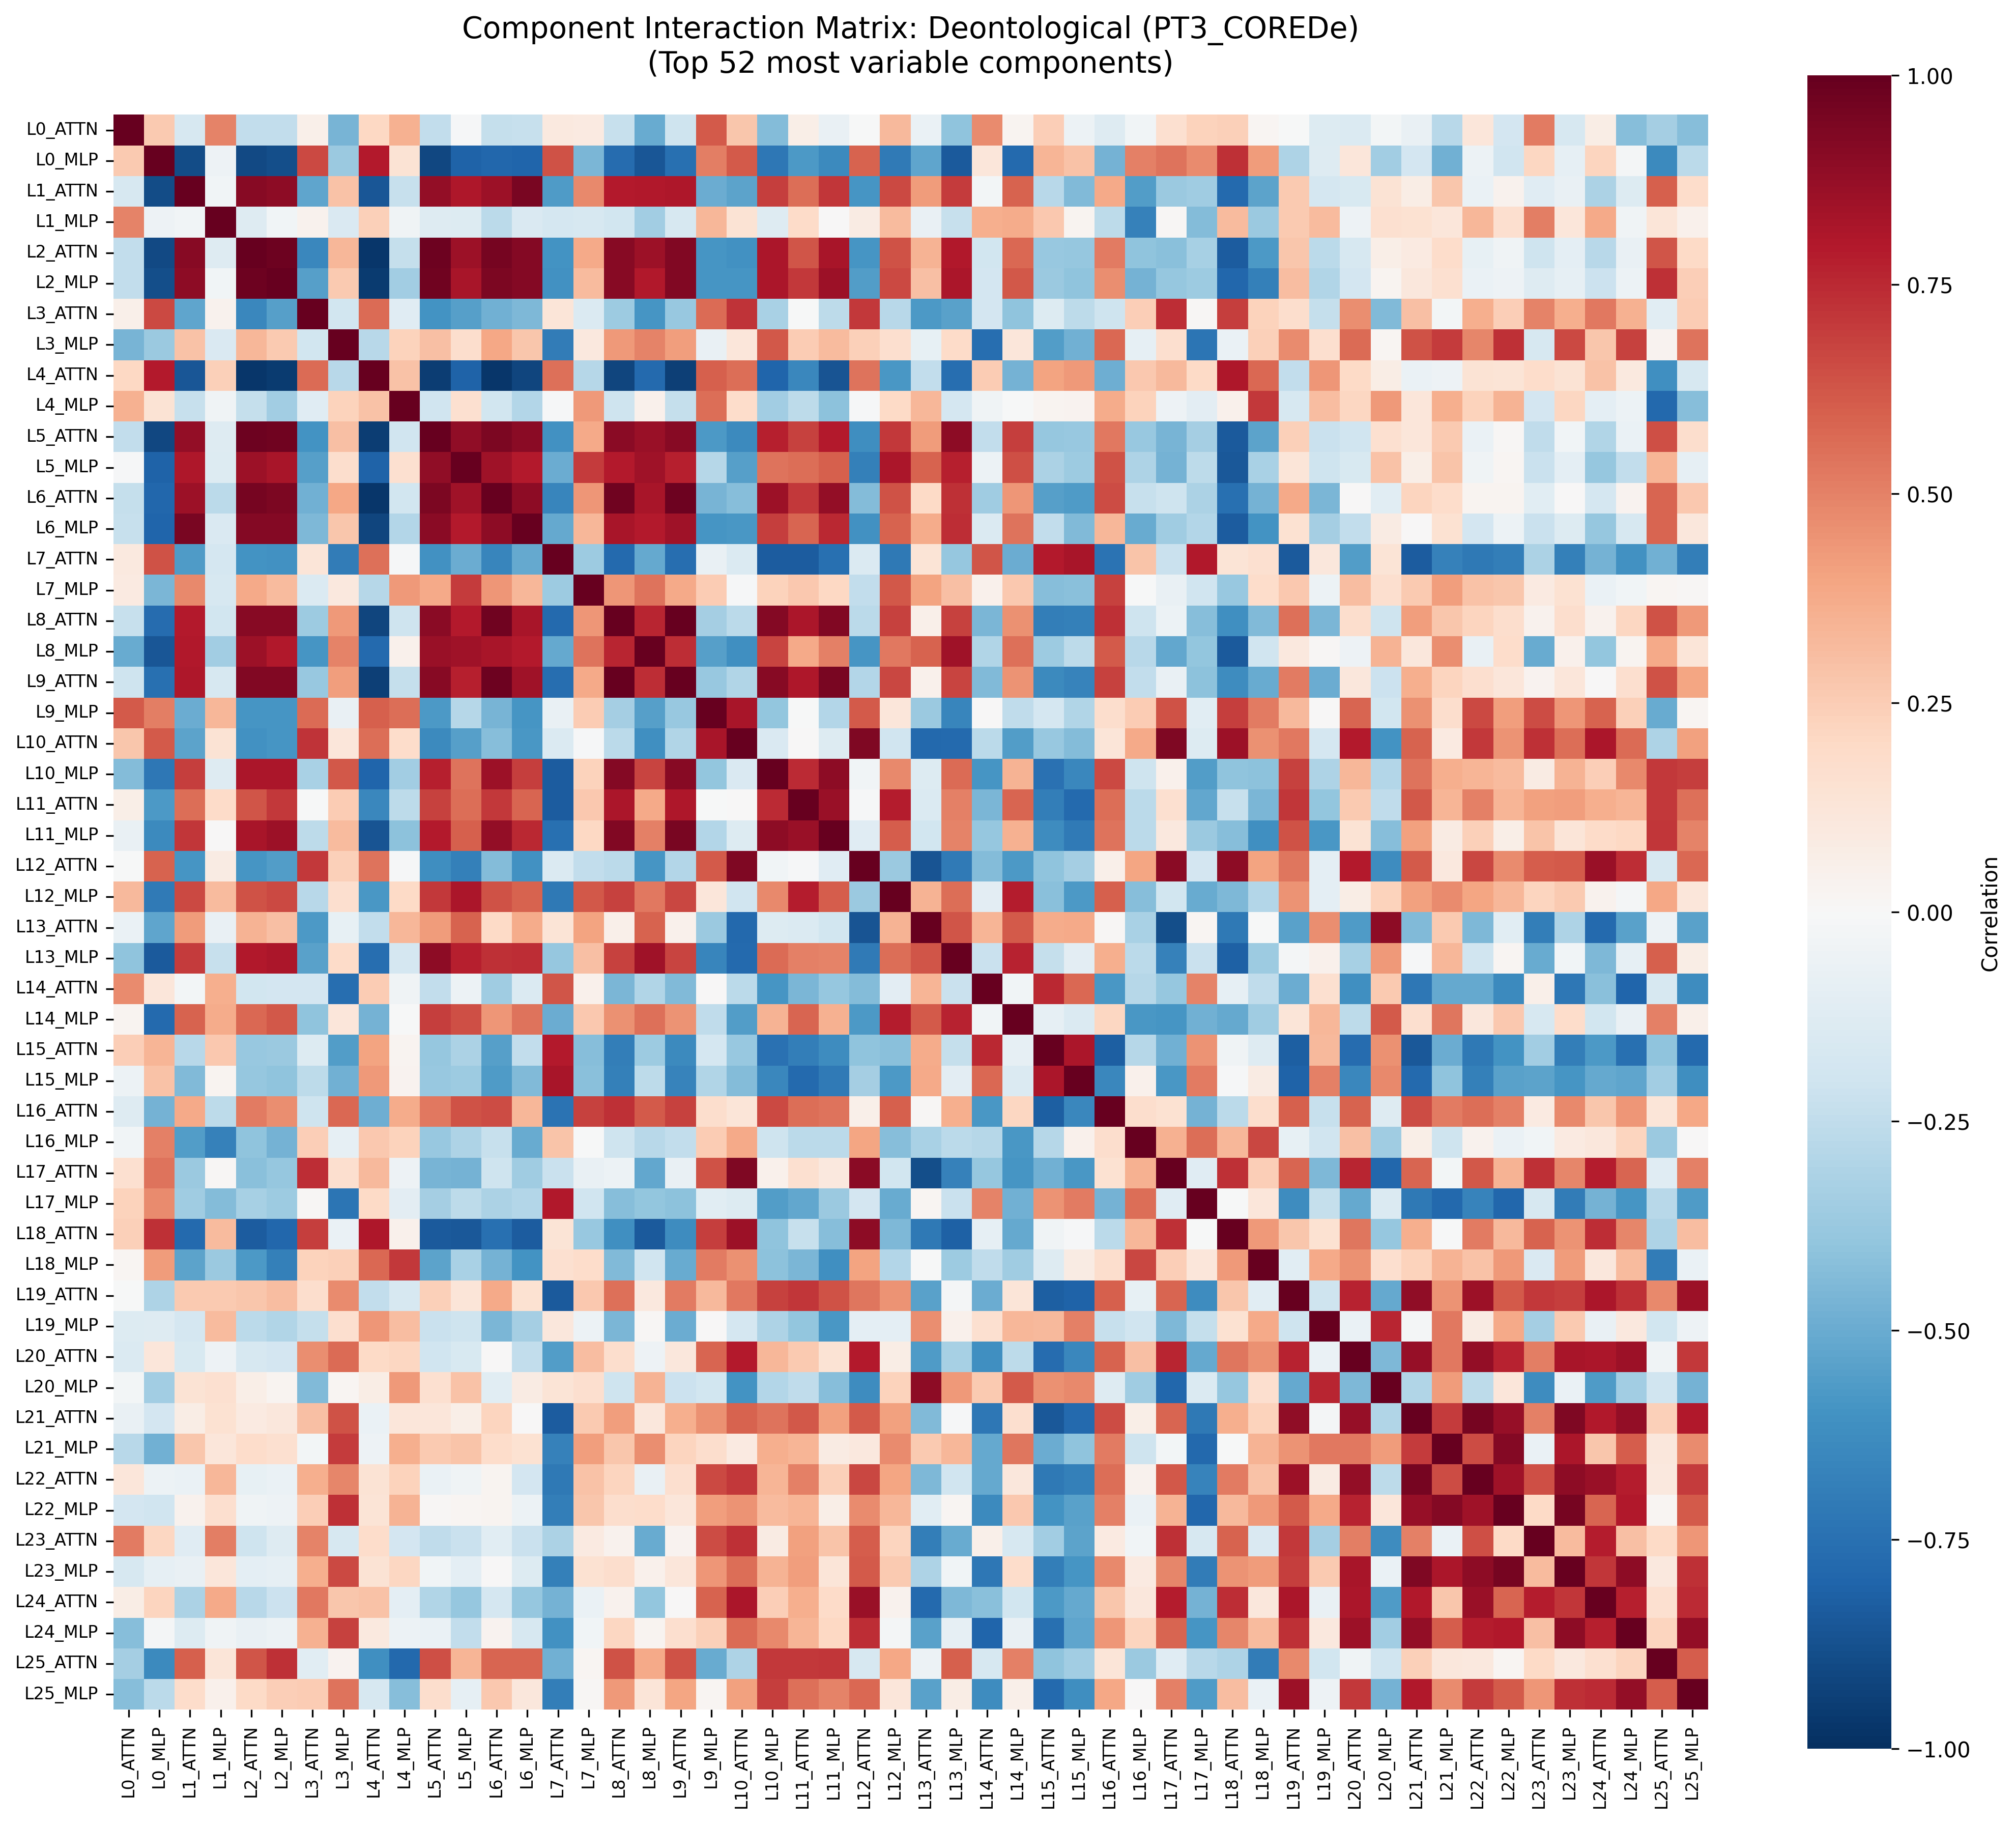
\includegraphics[width=\linewidth]{../mech_interp_outputs/component_interactions/correlation_matrix_PT3_COREDe_chronological.png}
    \caption{Deontological Model Interaction Matrix}
  \end{minipage}
  \hfill
  \begin{minipage}{0.48\textwidth}
    \centering
    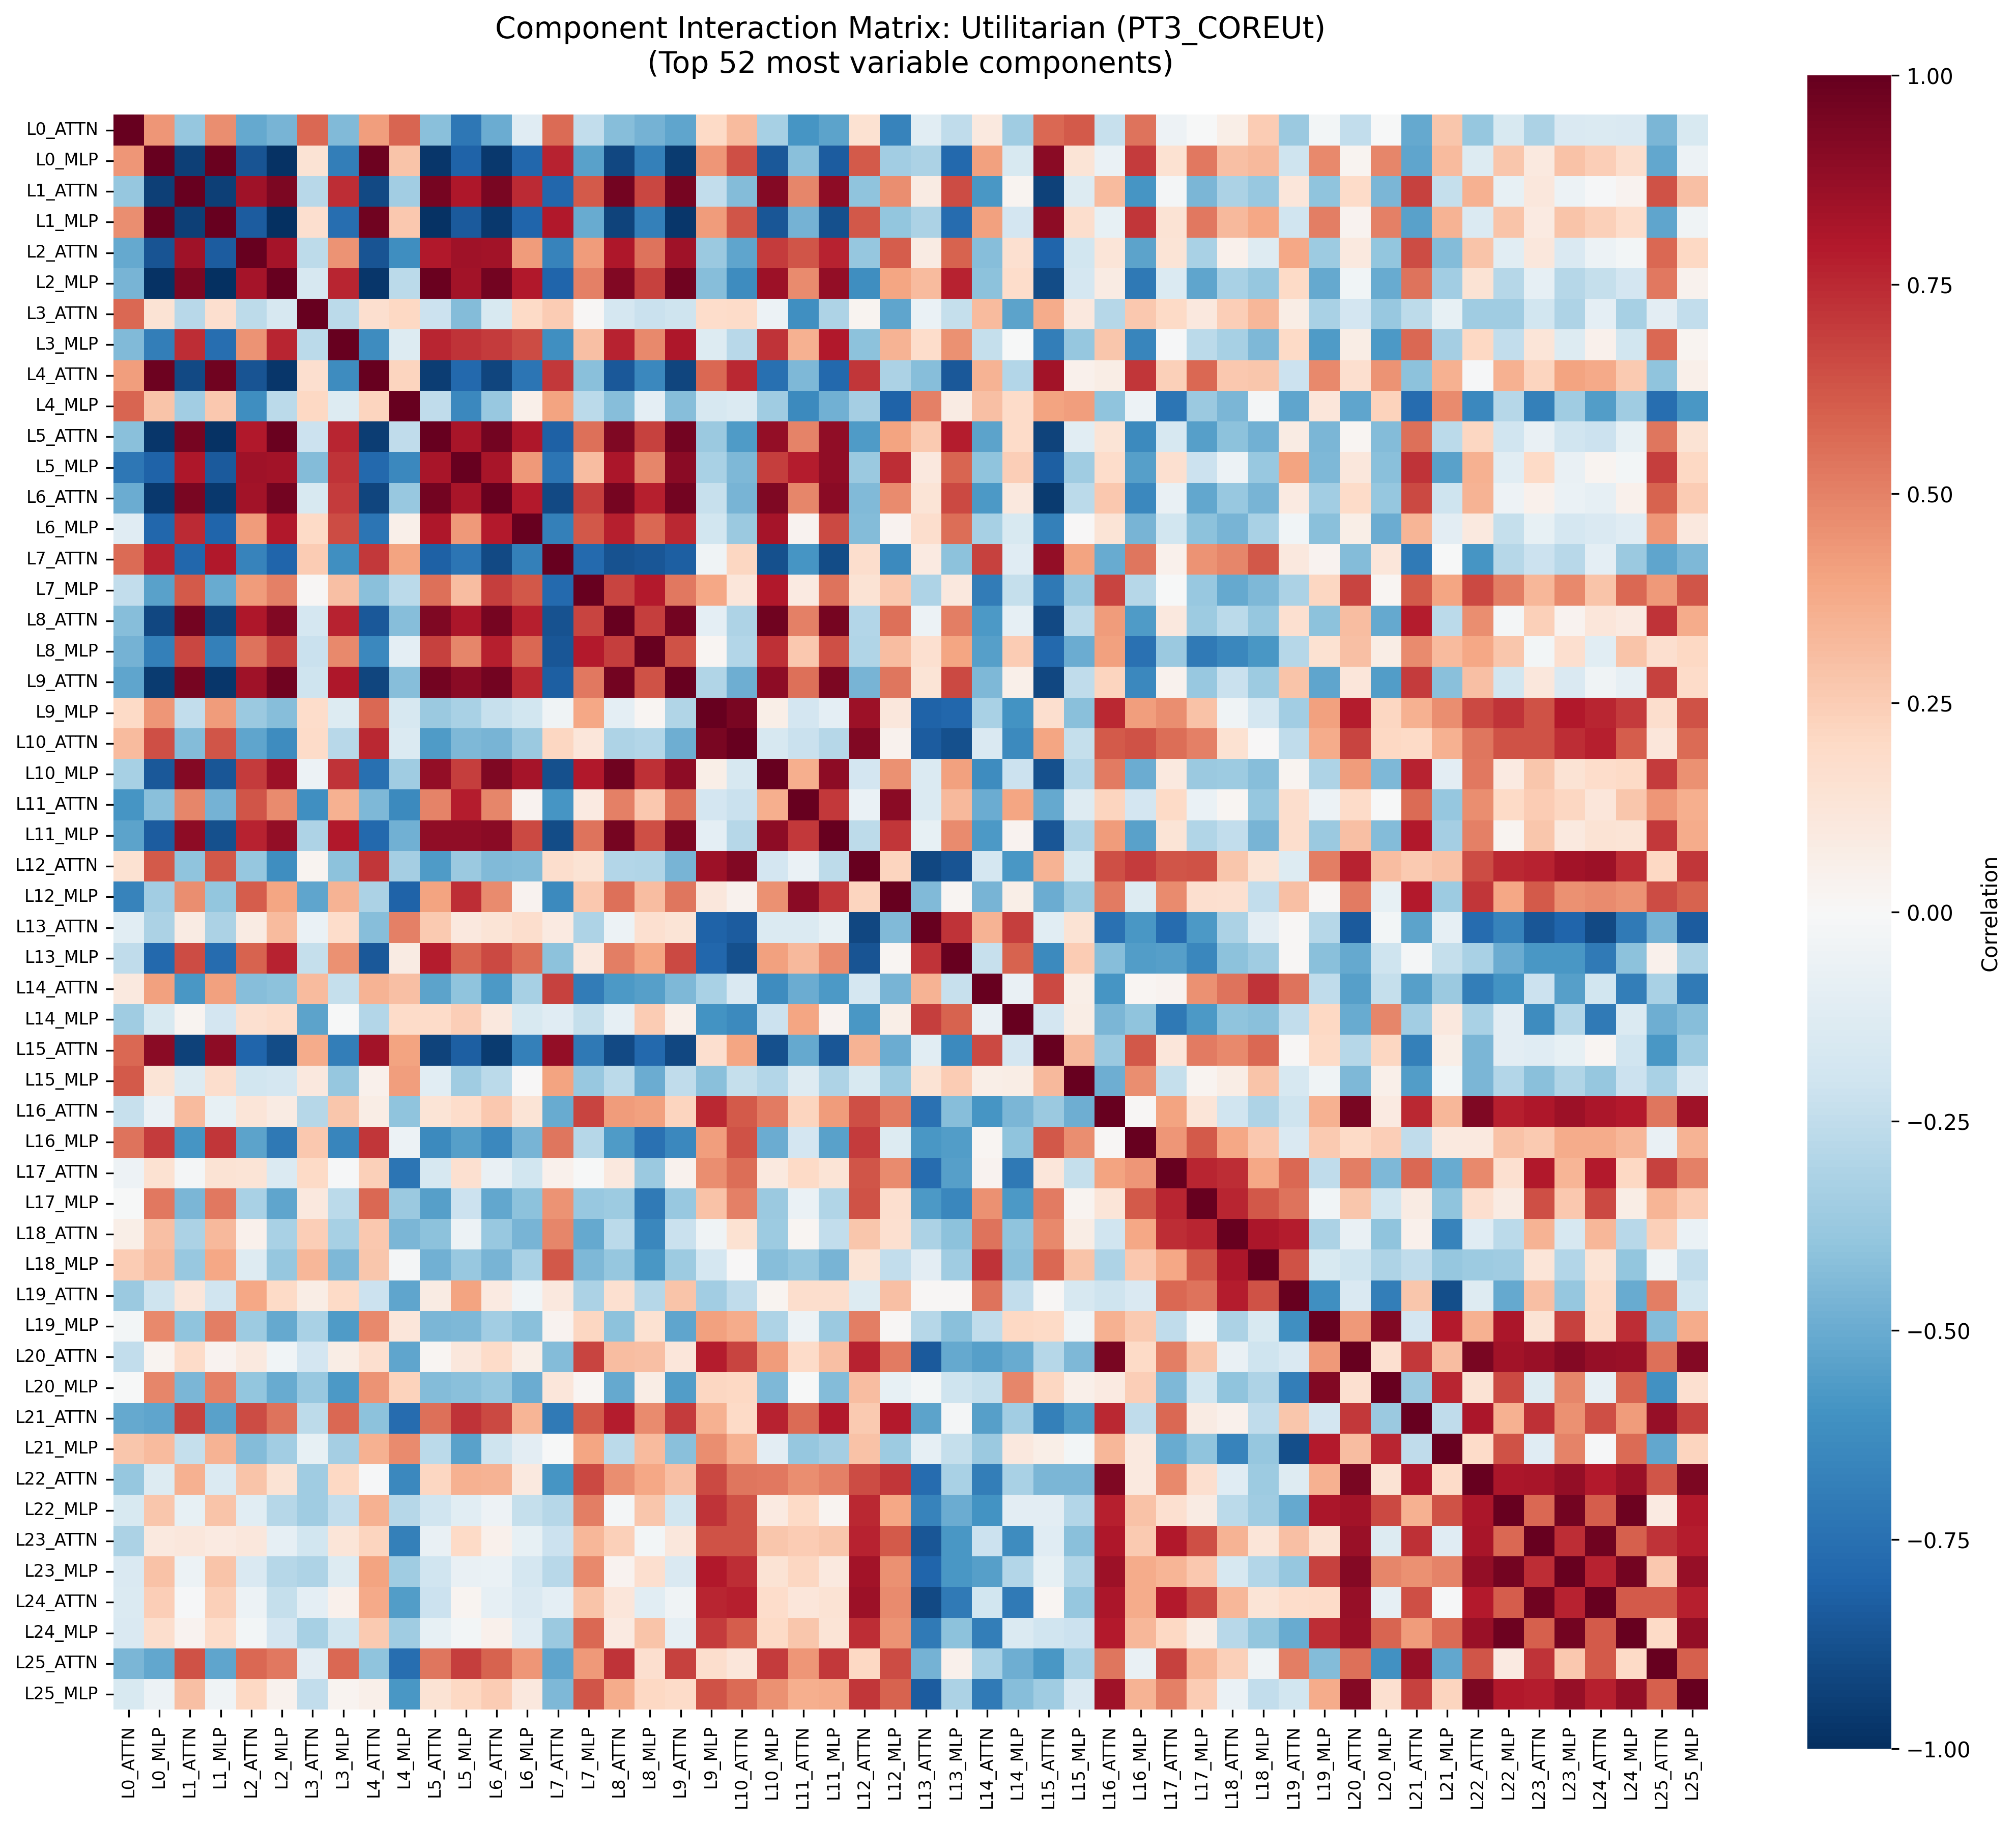
\includegraphics[width=\linewidth]{../mech_interp_outputs/component_interactions/correlation_matrix_PT3_COREUt_chronological.png}
    \caption{Utilitarian Model Interaction Matrix}
  \end{minipage}
  \label{fig:raw_matrices}
\end{figure}

While both matrices exhibit similar large-scale structure (e.g., strong positive correlations along the diagonal corresponding to neighboring processing), subtracting them yields the correlation difference heatmap (Figure \ref{fig:rewiring}) which highlights the specific diverging pathways.

\end{document}